\chapter{CMOS MAPS sensors} \label{ch:CMOS}

The fourth chapter aims to introduce the essential features of the semiconductor detector technology, going through the history of its advancements, which have led to the currently most promising sensors based on CMOS logic structure, the Monolithic Active Pixel Sensors (MAPS). The VTX program wants to make the most of the technologies that have already proven reliable in precision measurements, ensuring fast readout and high radiation tolerance, like the TJ-Monopix development line. We will briefly present it, mentioning the peculiarities of its prototypes, to better understand how they could fulfill the Belle II requirements.


\section{Semiconductor detectors} 

The detection of elementary particles, nuclei and radiations occurs through their interaction with matter. In particular, charged particles are often detected by atom ionization or excitation of the sensitive detector layers along their path passing through. This detection method can be used in gases, liquids and semiconductors. We want to focus on detectors that use semiconductors as sensitive material. \\

All solids can be divided into three categories based on their electrical conductivity: conductors, semiconductors and insulators. 
In a solid state lattice, the constituent atoms have a dense periodic arrangement and the energy levels of some level groups lie energetically so dense (order of meV) that one speaks of \emph{energy bands}, separated from each other by a \emph{band gap}, which represents the distance in energy between them (\textbf{$E_{G}$}, energy gap). The electrical conduction properties of materials are determined by the two highest energy bands, which are the \textbf{valence band (VB)} and the \textbf{conduction band (CB)}. The energy levels within the same band are so close that the transitions to unoccupied levels, if they are not completely filled, are easly possible. Therefore the electrical conduction properties depend on the band gap between the two levels and on the band occupation, as we can see in~\autoref{fig:energy_band}.

\begin{figure}[h!]
\centering
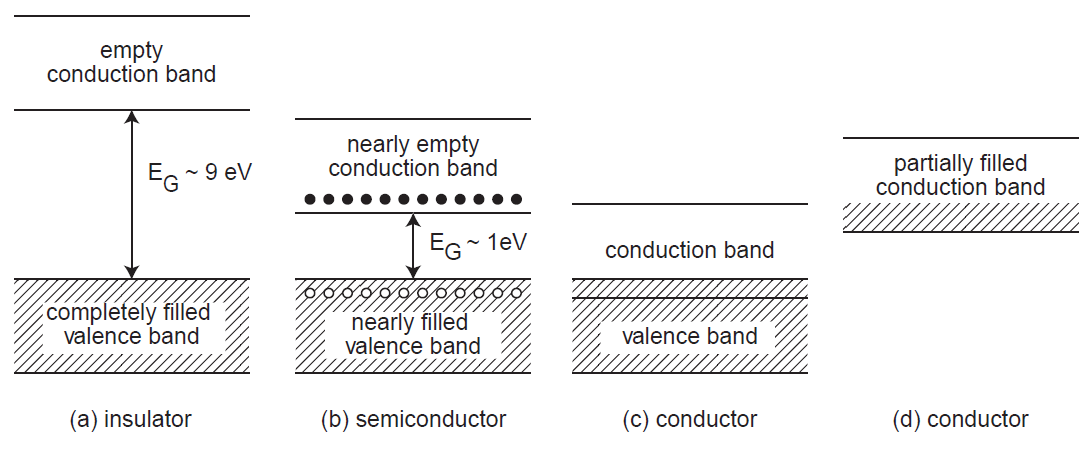
\includegraphics[scale=.6]{energy_band}
\caption{Schematic structure of the energy bands in insulators (a), semiconductors (b) and conductors (c,d).}
\label{fig:energy_band}
\end{figure}

In insulators the valence band electrons are strongly bonded to neighbouring atoms, they are not free and they do not contribute to the conduction. In fact the VB is entirely occupied, the CB instead, is empty. As a consequence of the strong interatomic bond, there are large energy gaps between the VB and the CB (typically $E_{G}$ of about \SI{9}{GeV}). Thus current flow is pratically impossible. 

In semiconductors weaker bonds between neighbouring atoms result in a smaller energy gap with respect to the insulator (for example \SI{1.12}{eV} in silicon). In this way electrons from VB can easily overcome the gap, moving on the CB by thermal excitations or by external electric fields. When an electron makes this transition, it leaves a hole in the VB, wihch could be filled in turn, by another electrons of the VB. Applying an external electric field, the free electrons in the CB and the holes in the VB start to move producing two different current flows, one negative and the other positive, respectively.

In conductors, either the conduction and valence bands overlap or the conduction band is partially filled, so transitions within the same band and between the two different bands are easy and current conduction requires minimal energy.


\subsection{Movement of charge carriers and signal formation in semiconductors}

Semiconductor materials are the only ones that allow the detection of charged particles by ionization of the sensitive matter (in conductors a current is always present, not only in case of particle or radiation crossing). 

When a charged particle or a photon pass through the medium, they release a certain amount of energy mainly by ionization, atom excitation and bremsstrahlung radiation the first, absorbtion by semiconductor the second. Most part of this energy loss, in turn, causes the formation of positive and negative charges, which in this context, are defined charge carriers (the rest is absorbed by the lattice). In semiconductors these carriers are the hole electron pairs created by ionization, which start to move in opposite direction due to an external electric field: the holes (positive) migrate towards the \textit{\textbf{catode}} and the electrons (negative) towards the \textit{\textbf{anode}}, which sense the signal induced by this movement. In fact, their drift induces an accumulation of charges on the electrode surfaces, and it is possible to record this charge induction as a charge, current or voltage signal. It is worth to notice that the generation of the signal depends on the movement of the carriers relative to the electrodes, and not when they actually arrive, that is the moment in which the signal stops.\\

The charge carrier density of semiconductors can be modified by doping the material with specific chemical elements, and this process causes a modification of their conduction properties.
Undoped semiconductors are called \emph{intrinsic semiconductors}. \\
\emph{Extrinsic semiconductors} instead, are artificially doped with external impurities like: 

\begin{itemize}
\item Pentavalent elements (P, As, Sb), called \emph{donors}, added in a tetravalent material (Si, Ge) produce an excess of conduction electrons with respect to the holes (n doping, \autoref{fig:doping} (a)).
\item Trivalent atoms (B, Al, Ga), called \emph{acceptors}, create an excess of holes (p doping, \autoref{fig:doping} (b)).
\end{itemize}

\begin{figure}[h!]
\centering
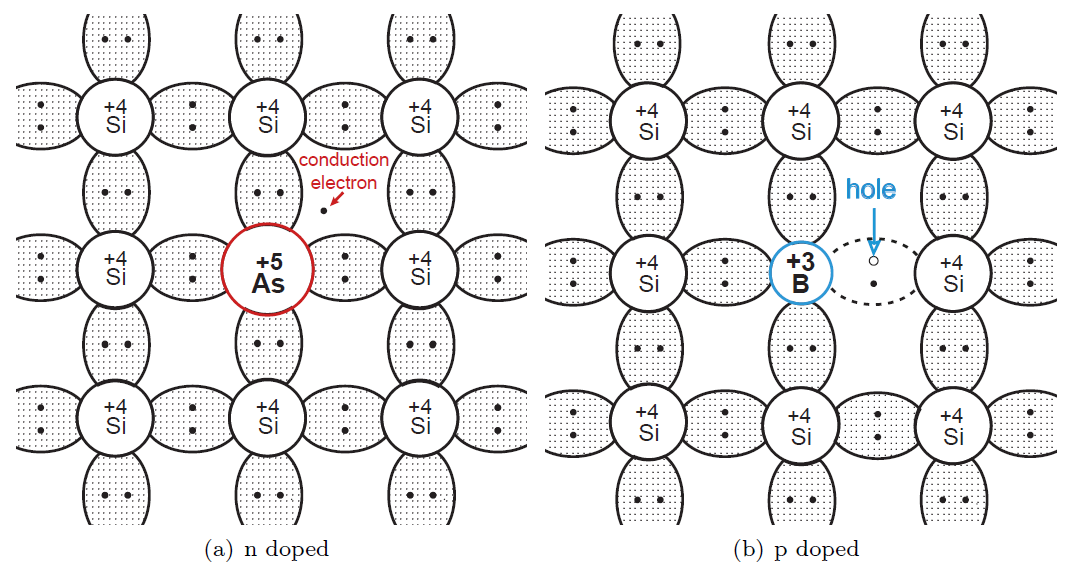
\includegraphics[scale=.5]{doping}
\caption{Schematic representation of atom bonding structure in n-doped and p-doped semiconductors.}
\label{fig:doping}
\end{figure}


\subsection{The pn junctions as detector}

The base material employed in semiconductor detectors is silicon, because it is stable, abundant and it has a low band gap which allows to produce an adequate amount of charge to be detected.\\ 
When a p-doped semiconductor get in contact with a n-doped material, a \textit{pn junction} is formed. In particular, the p-doped part is the one where holes are the dominant charge carriers, called \textbf{majority carriers}; in the n-doped part of the crystal instead, the majority carriers are the electrons. 
The presence of these excesses of opposite charge in the two parts of the junction, generates a potential difference across the junction, which causes a migration of the majority carriers from each part to the opposite one. At the boundary the charges recombine (when a conduction band electron occupies a valence band hole, losing energy), and this process creates a zone which is free of charge carriers, called \textbf{depletion zone}. After the recombination, the atoms of this depletion region are ionized, and so it is no longer neutral, but features a \emph{space-charge}(\autoref{fig:space_charge}): a positive one in the n-layer, and negative in the p-layer. Moreover these space charge densities are opposite in sign, so they generate an intrinsic electric field that stops the original diffusion.\\

\begin{figure}
\centering
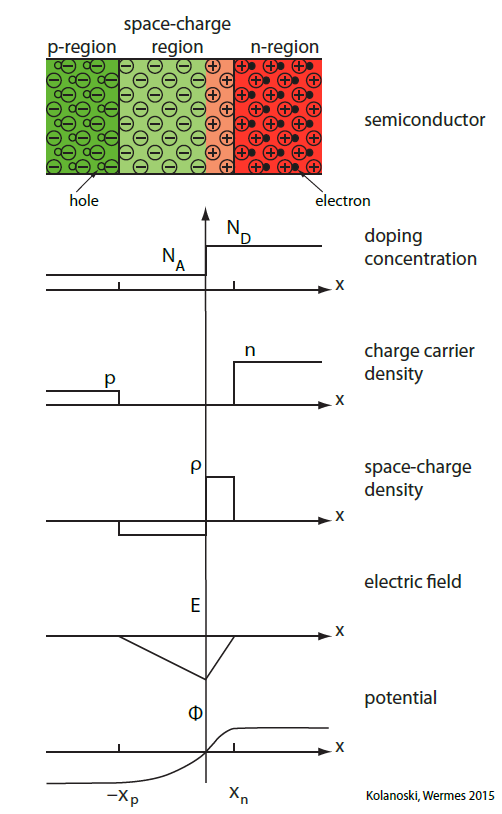
\includegraphics[scale=.5]{pn_junction}
\caption{Doping concentration, charge carrier and space charge densities, electric field strength and electric potential in a p-junction.}
\label{fig:space_charge}
\end{figure}

Moreover, the application of an external voltage $V_{ext}$ between the two sections of the junction, provokes a variation of the width of the depletion region, depending on the size and polarity of the applied voltage. It is possible to distinguish:%~\autoref{fig:bias}:

\begin{itemize}
\item \emph{forward bias}, $V_{ext}$>0: a positive external voltage applied to the p side with respect to the n side, causes a reduction of the depletion region;
\item \emph{reverse bias}, $V_{ext}$<0: if a negative voltage at the p side or positive at the n side relative to the respectively opposite side is applied, the depletion region gets wider.
\end{itemize}

\begin{comment}
\begin{figure}
\centering
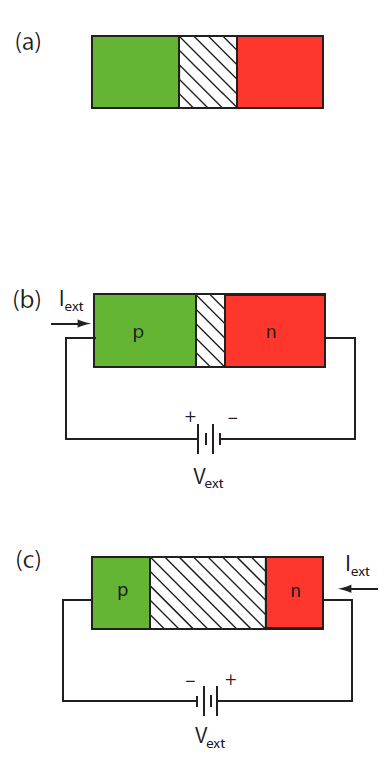
\includegraphics[scale=.5]{depletion}
\caption{A pn-junction without external voltage in (a), with forward voltage applied in (b), and with reverse voltage applied in (c).}
\label{fig:bias}
\end{figure}
\end{comment}

Depleted region is a zone without free charge carriers (do not come from the signal), and with the presence of an external eletric field (reverse bias), it is a fundamental for semiconductor detectors.

The performance of the junction as a detector is determined above all, by the boundary properties between p-and n- doped silicon. Boundaries of the same doping type, but with different concentration, also create a similar pn structure, like for example $n^{+}n$ or $p^{+}p$. There are also Metal-semiconductor boundaries, used in metal contact with the outside and Metal-Oxide-Semiconductor interfaces (MOS) that we will see in more details in the following.
 
 
\subsection{Metal-Oxide-Semiconductor (MOS)}

A MOS structure is a double interface made of three different media: an insulator (oxide) placed between the metal and the semiconductor, as shown in~\autoref{fig:mos}.

\begin{figure}[h!]
\centering
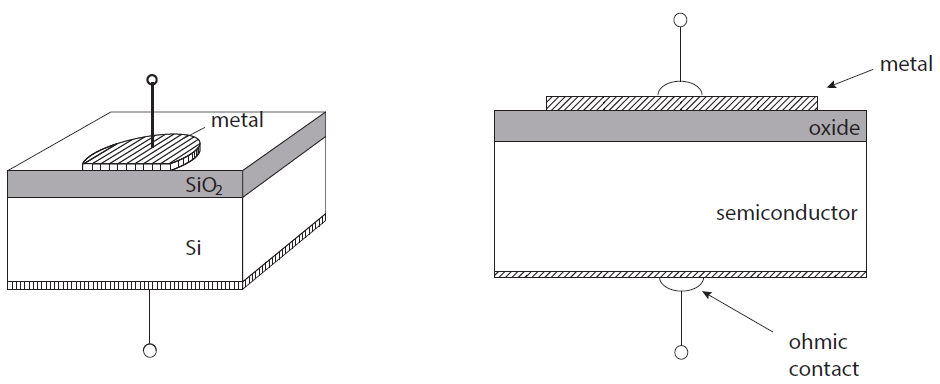
\includegraphics[scale=.6]{mos}
\caption{A perspective (on the left) and a cross-sectional illustration (on the right) of a MOS structure.}
\label{fig:mos}
\end{figure}

In recent transistor technology, the metal is almost entirely replaced by highly doped polysilicon, like $n^{++}$ and $p^{++}$ since these materials are more resistant to high temperature. Despite this, the physics remains essentially the same. 
The MOS structure plays a very important role in chip electronics, including the readout of detectors, which employ a combination of NMOS and PMOS transistors, embedded in the substrate . This is st the base of the \emph{Complementary} MOS (CMOS) electronics, which allows to develop more complex circuits. This technique consists in accomodate one of the two transistor type in a differently doped area, called \emph{well}. For example,  in a p-type substrate, a PMOS transistor are accomodate in n-wells, and vice versa with a n-type substrate. 


\section{Hybrid and monolithic pixel sensors}

Nowadays the most important sensors used as tracking detectors are the semiconductor detectors, expecially at high rates and high radiation levels. We have already seen that the particle passing through semiconductors, releases energy producing electron-hole pairs in the depletion region, which in turn, are separated by an external electric field. Moreover, the signal produced depends on the number of pairs generated, the carriers velocity drifting towards the electrodes, and the electrode geometry. 
In particular, the drift velocity depends on the carge carrirers mobility, which is a function of the electric field, and on the electric field applied (Drude model):

\begin{equation}
v_{D} = \mu(E) E
\end{equation}

At high electric field values, the mobility starts to saturate.
Spatially sensitive semiconductor detectors, like miscrostrip or pixel detector, are usually very thin (200 - \SI{300}{\micro m}) with typical velocities of about \SI{50}{\micro m/ns}. So the time needed to pass trough the space charge region is of $\approx$ 4-\SI{6}{ns}. 

There are several type of semiconductor detectors which are distinguished from their geometry, their micro-structure, their arrangement and other features. We want to see in more details, two among them: \emph{hybrid} and \emph{monolithic} pixel sensors, where the sensor and the readout could be separate entities or integrated in the same silicon crystal, respectively.


\subsection{Hybrid pixel detector}

Differently from \textit{monolithic} sensors, \textit{Hybrid} pixel detectors are composed by two different parts: a silicon layer structured in pixel cells, which represents the pixel sensor, and the readout chips with the same cell pattern, that process, digitize, store and transmit the hit data. At each pixel, they are connected by a conducting microconnection (called \emph{bump bond}). In~\autoref{fig:hybrid} is shown an example of a detector module. 
%There are different bonding techniques which allow to connect the two layers, like \emph{bump-bonding}, \emph{flip-chipping} and \emph{3D integration}. 

\begin{figure}[h!]
\centering
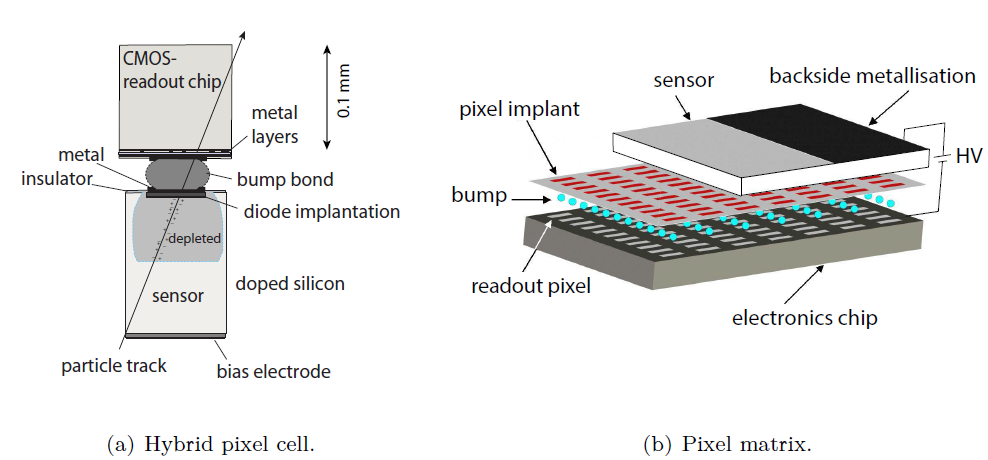
\includegraphics[scale=.6]{hybrid}
\caption{On the left (a), the structure of a single pixel cell, made by the sensor and the electronic readout. On the right (b), an exploiting representation of the entire hybrid pixel matrix arrangement.}
\label{fig:hybrid}
\end{figure}

When a particle crosses the sensor, a signal is generated on the electrodes due to the drift of the charge carriers in the depleted region. This signal passes through the conductive bump in the readout chip, where it is amplified and discriminated.

One of the advantage of the pixel detectors with respect to the strip sensors, is the higher tolerance to radiation damage. The \emph{leakage current} increses as the radiation doses become higher, it depends on the volume of the sensors and it is distributed over all the electrode. In pixel detectors this current is shared among more electrodes with respect to the strip detectors, so the leakage current per electrode is smaller. Moreover, as separate entities, sensor and readout could be independently optimize.

Among the disadvantages instead, there are the cost and complexity of the implementation processes, but also large material thickness together with the necessity to add support and cooling structures, which worsen the track reconstruction and momentum resolution because of the multiple scattering.


\subsection{Monolithic pixel detector}

We have seen that hybrid detectors are made by the active sensor and the passive readout chip in two separate structures, connected by micro-connections. Since both of them are made of silicon, in principle, it could be possible to build them in a monolithic unit. In this way the amount of material decreases, enhancing the tracking performance and momentum resolution. 

Developments of this sensors have tried to exploit industrial technologies already available, like the CMOS technologies. They have to reach a large depletion zone in order to improve the signal-to-noise ratio, but also design electrode with small capacitance, to reduce the power consumption and the noise. High radiation tolerance is also required.

An example of this type of sensor is the DEPFET pixel detector, which contains only one active transistor in every pixel. Monolithic Active Pixel Sensors (MAPS) employed CMOS technologies to include a readout circuit in their structure and we will see them in more details in~\autoref{sec:MAPS}

\begin{description}
\item[Depleted p-channel field effect transistor (DEPFET)]
\end{description}

In a DEPFET pixel detector, each pixel implements only one transistor. In~\autoref{fig:DEPFET} is shown an example of a DEPFET pixel.

\begin{figure}[h!]
\centering
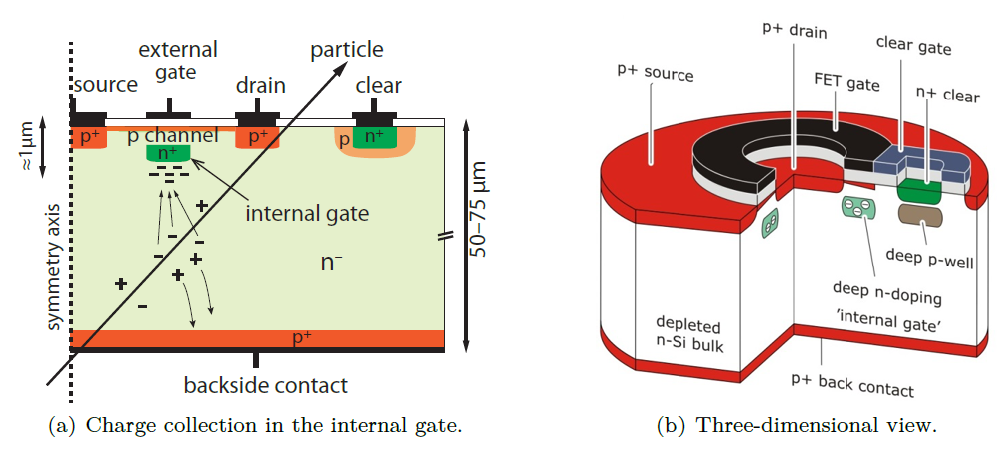
\includegraphics[scale=.6]{DEPFET}
\caption{On the left (a) a cross section of a circular DEPFET pixel cell, where the charge collection is also sketched. On the right (b), a three-dimensional view of the same pixel cell.}
\label{fig:DEPFET}
\end{figure}

The depletion region extends between the backside $p^{+}$ contact and the several $p^{+}$ regions near the transistor element (drain, source and a $n^{+}$ clear contact installed in a p region) and the $n^{-}$ substrate. When a traversing particle releases energy, ionizing the medium, electrons drift towards the top surface, and the holes towards the backside due to the external potential.\\
The transistor is a p-channel MOSFET that produces a hole current from source to drain, controlled by the potential on the external gate. In addition, there is a deep $n^{+}$ implant placed a few micrometers under the transistor. It is the most positive point in the pixel structure and so it is a local minimum for the electrons. In fact this implant features an electron accumulation, which changes the potential making it an \textit{internal gate}. 
Electrons collected on this electrode, and the external gate influece the current flow in the DEPFET transistor channel. After the measurement, they are removed applying a positive voltage on the \textit{clear contact}. In order to not compete as a collection electrode for the electrons, this element is embedded in a p region (\textit{deep p-well}).\\
With some variations in the pixel structure, this is the type of sensors that PXD is made of.


\section{CMOS Monolithic Active Pixel Sensors technology} \label{sec:MAPS}
 
First prototypes of pixel detector, which employed the CMOS technology to fabricate both the sensor and the readout circuit in the same silicon die, date back to the early 1990s. Further developments have led to the \emph{monolithic active pixel sensors} (MAPS) with an epitaxial silicon layer for charge collection and then to the Depleted MAPS (DMAPS), where the depleted region is extended throughout the volume.

\subsection{MAPS pixel detectors}

This type pf sensors have been exploited the CMOS tehnologies for optical application, where the structure have an epi-layer with high resistivity to detect the light, and the electronic circuitry on the top of it. In this case, not the entire area is sensitive to the charge production. The effectively active fraction of the pixel area is called \textbf{fill factor}. 
In~\autoref{fig:MAPS_fig} is shown a schematic of their structure. 

\begin{figure}[h!]
\centering
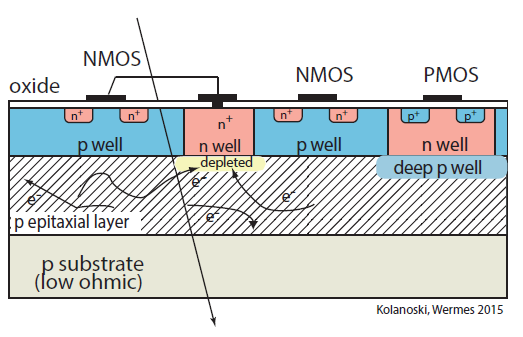
\includegraphics[scale=.7]{MAPS}
\caption{Schematic of a monolithic pixel detector (MAPS).}
\label{fig:MAPS_fig}
\end{figure}

In MAPS pixel detector, charge collection is mostly achieved by diffusion, because the sensitive region is not fully depleted. The collection electrode is a $n^{+}$ contact in a n-well, embedded in a p-epitaxial layer put on the top of a p substrate. Other n-wells can be necessary, for example to host PMOS transistors, and for this reason they have to be shielded by deep p-well, to prevent them to become competitive for charge collection. These highly doped deep layers assume a negative potential with respect to the collection electrode and hence a repulsive effect.
Due to the absence of a drift field in the epi-layer, with the exception of the region immediately below the collection electrode, collection charge occurs mainly by diffusion and thus it is slow and incomplete. 
Typical values of the epi-layer thickness are within the range of 1 - \SI{20}{\micro m} \cite{Garcia-Sciveres:2017ymt}.

These MAPS detector cannot be used in high rates experiments because they have charge collection time of the order of \SI{100}{ns}, thus too slow. The signal in this standard process is very small (typically $\geq$ 1500 $e^{-}$), due to the small thickness of the epitaxial layer, not even fully depleted, and they also have limited radiation tolerance. 
In fact due to Non-Ionising Energy Loss (NIEL) effects \cite{wermes_book2020}, radiation produces displacement damage in the sensor bulk also creating energy levels in the band gap that acts as trap centers. 
Electrons and holes can be trapped and then be released again after some time. This produce a decrease of the signal amplitudes if the de-trapping time constant is longer than the time of signal formation. 

Although their limited radiation tolerance MAPS sensors have been successfully employed for heavy ions collisions, like STAR experiment at RHIC (Relativistic Heavy Ion Collider) \cite{Greiner:2013tva} and the ALICE upgrade at the LHC \cite{ALICE:2013nwm}.


\subsection{Depleted MAPS pixel detectors}

In order to obtain fast and fully collection of released charge, it is necessary to drift the carriers toward the electrodes, by an external electric field. A fully depletion of the sensitive zone enhances the charge collection, producing large signal (thus a better signal-to-noise ratio). \\
The depletion depth depends on the substrate resistivity and the bias voltage, according to the relation:

\begin{equation}
d \propto \sqrt{\rho V}
\end{equation}

For this reason, new processing techniques have been employed to allow applying higher voltage or to process high-ohmic substrate wafers. Both of them are used to increase the depletion region underneath the collection electrode (typically to 25– \SI{150}{\micro m}) and so to provide sufficiently large and fast signal.

We can distinguish two main variants of DMAPS pixel detector \cite{Garcia-Sciveres:2017ymt}: with a \textit{large} or \textit{small} collection electrode, shown in~\autoref{fig:fill_factor}.

\begin{figure}[h!]
\centering
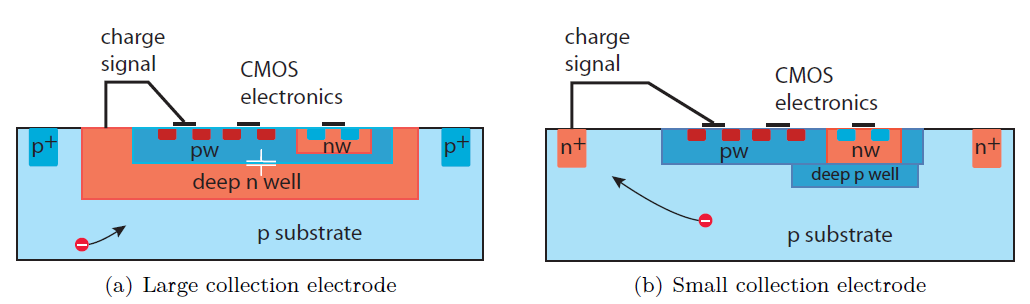
\includegraphics[scale=.6]{fill_factor}
\caption{On the left (a) a schematic of the large electrode design. On the right (b) the small electrode design.}
\label{fig:fill_factor}
\end{figure}

The \textit{large collection electrode} DMPAS features a deep n-well acting as electrode but also as shield for the entire CMOS electronic readout, which is embedded within it. This architecture improves the radiation tolerance because the reduced average drift distance of the charge carriers decreases the probability of trapping. At the same time though, large size of the electrode implicates higher values of capacitance (several hundred fF) which increases the noise and worsens the timing performance.\\
The \textit{small collection electrode} variant has a small n-well collection node, distanced from the CMOS circuitry which is embedded in p-well and deep p-well layers. In this design, low capacitance of about 5-\SI{20}{fF} can be obtained, improving noise and timing performance.
Radiation tolerance instead, is more difficult to reach due to larger average distance travelled by the carriers. Smaller pixel dimensions are preferred for small electrode (to reduce the path), and therefore higher power density is accepted in exchange of increased robustness against radiation.\\


\begin{figure}[h!]
\centering
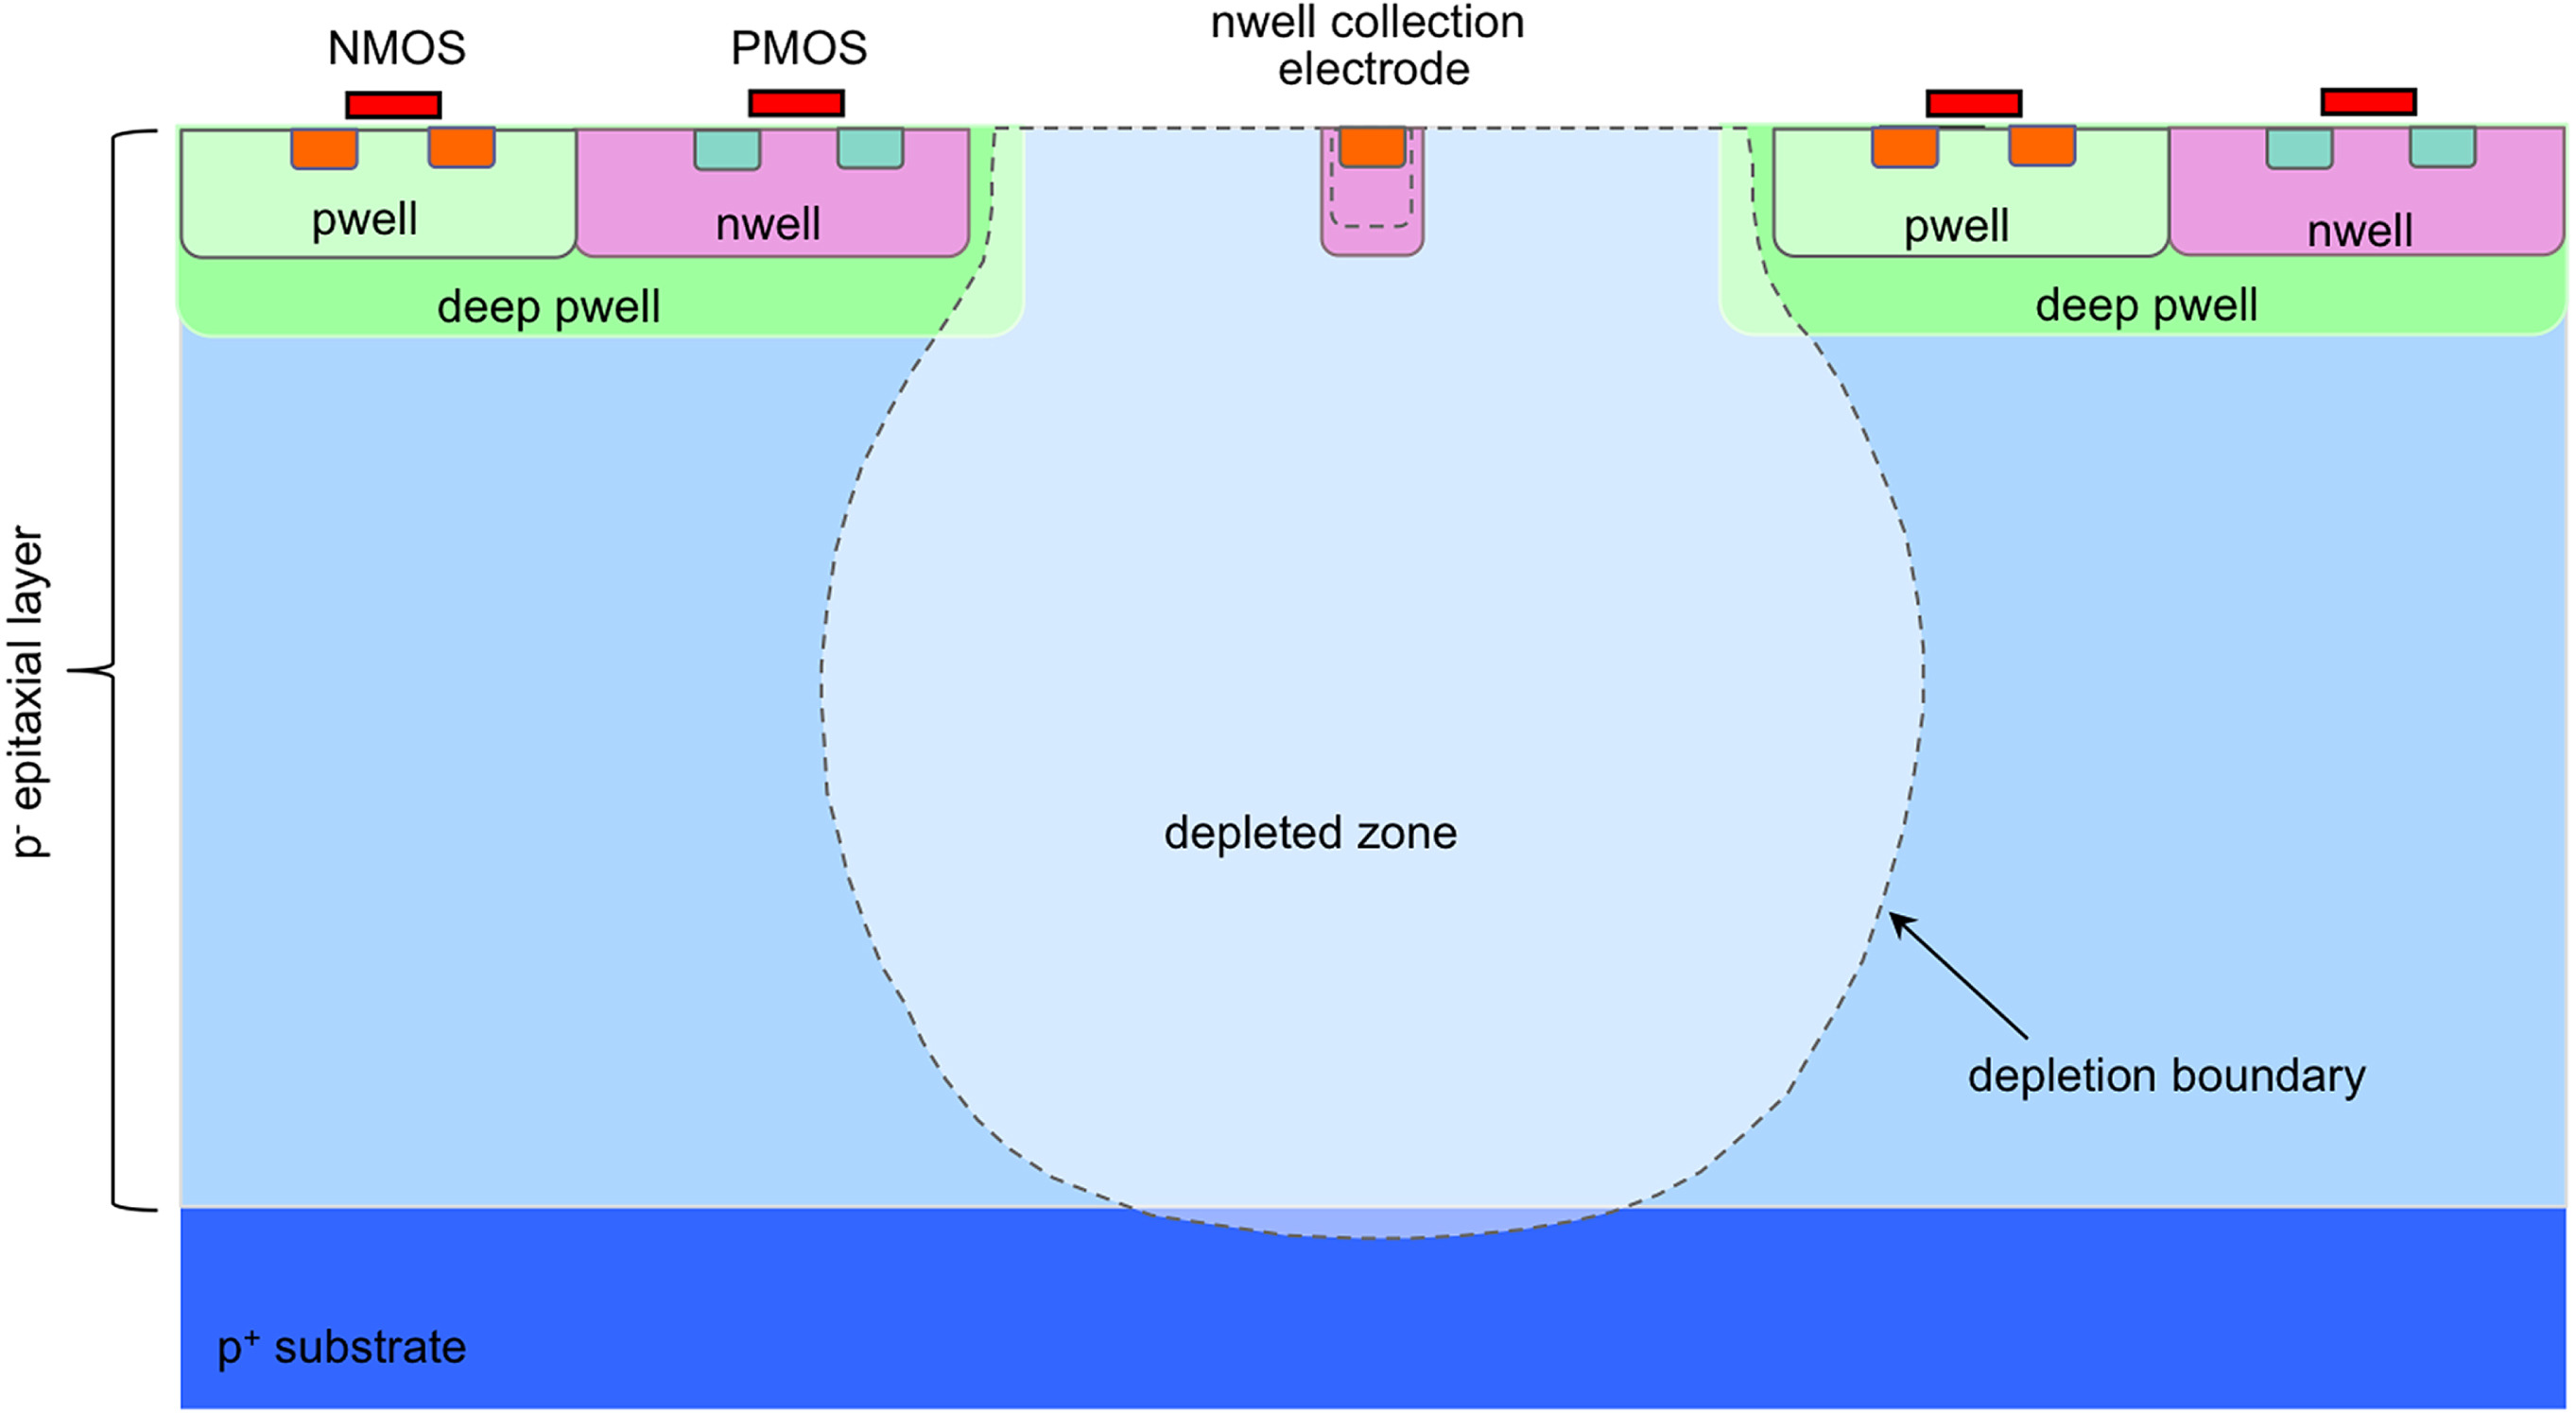
\includegraphics[width=.45\textwidth ,keepaspectratio] {alpide_process.jpg}
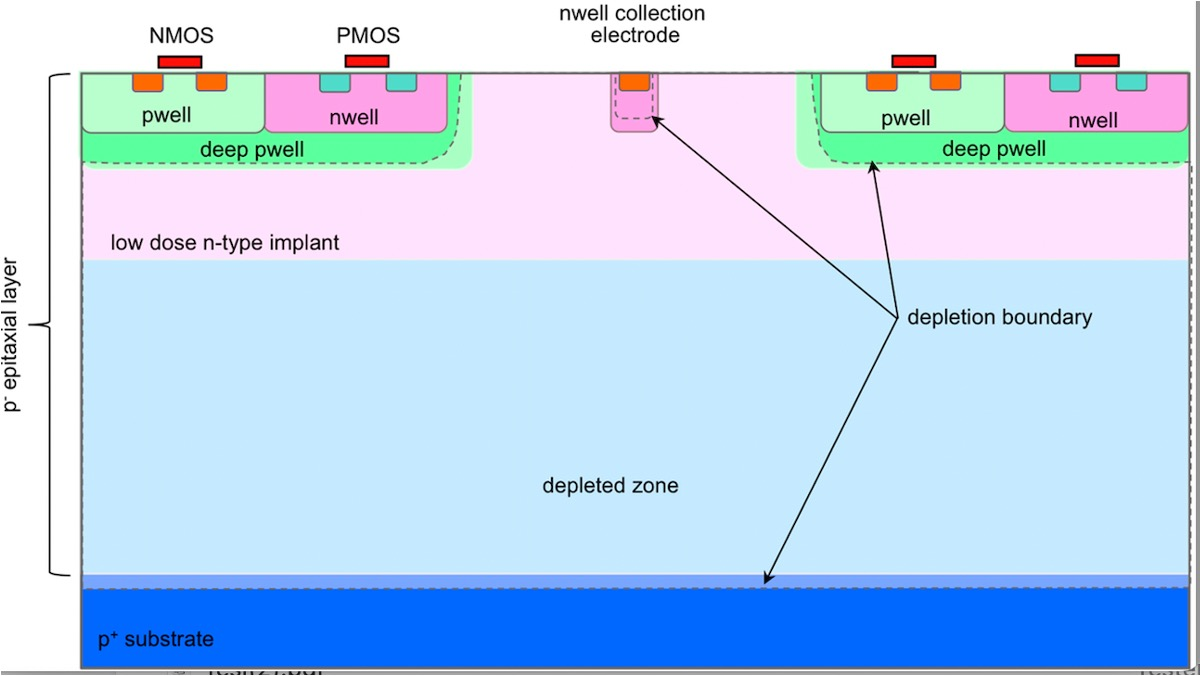
\includegraphics[width=.45\textwidth ,keepaspectratio]{modified_process.jpg}
\caption{Small electrode design adopted in the ALPIDE sensor with the standard process (left) and the process modification with the addition of a low dose n-doped layer used to implement a planar junction and deplete the epitaxial layer over the full pixel area.}
\label{fig:n_doped}
\end{figure}


In the standard process adopted for the ALPIDE sensor \cite{AGLIERIRINELLA2017583} it is difficult to deplete the epitaxial layer over its full width as it is shown in~\autoref{fig:n_doped} left side. 
In order to achieve the full depletion of the sensitive layer, combined with a low capacitance collection electrode, a planar junction separated from the small collection electrode has been implemented.  A low dose deep n-type implant has been used to realize a planar junction in the epitaxial layer within the pixel matrix below the wells containing circuitry, as shown in~\autoref{fig:n_doped}. 
The epi-layer is thus depleted from two pn junctions: the deep p-wells and the low dose n-implant, the n-implant and the p-epitaxial layer~\cite{SNOEYS201790}. This addition creates a potential minimum for electron collection underneath the deep p-well with a field direction towards the n collection well, thus strengthening collection of charges laterally\cite{wermes_book2020}. The epi-layer is \SI{25}{\micro m} thick and the collection electrode is on positive potential.
This modification of the technology has allowed to further improve radiation tolerance. \\

The most probable value (MPV) of the signal released by a Minimum Ionizing Particle (MIP) in the thin MAPS sensitive thickness ($\approx$ \SI{25}{\micro m}) is only about 2000 $e^{-}$. 

The small charge signal achieved in the thin epi-layer (typically 1600 $e^{-}$) becomes a sizable voltage signal (about \SI{50}{mV}) due to the small ($\geq$\SI{5}{fF}) capacitance according to dV = dQ/CD. Therefore voltage (rather than charge) amplification is employed for the readout of small electrode MAPS.



\subsection{Silicon On Insulator (SOI) technology}\label{sec:SOI_tech}

\textit{Silicon on Insulator} (SOI) technology represents another way to combine the sensitive region and the readout circuit in a single monolithic unit. In this architecture, the transistor is isolated by vertical trenches and is divided from the bulk by a $SiO_{2}$ layer, called \emph{buried oxide} (BOX).
An high resistivity bulk wafer allows to depleted the volum in the region below the BOX, in order to generate a large charge signal when a particle passes through the detector. The bulk and the CMOS electronics are connected by vertical connections, called \textit{vias}. \\
In~\autoref{fig:SOI_fig} is displayed a monolithic SOI pixel, with a doped volume placed between the CMOS circuitry and the BOX. This variation prevents the capacitive coupling from the substrate into the electronics, through the BOX.

\begin{figure}[h!]
\centering
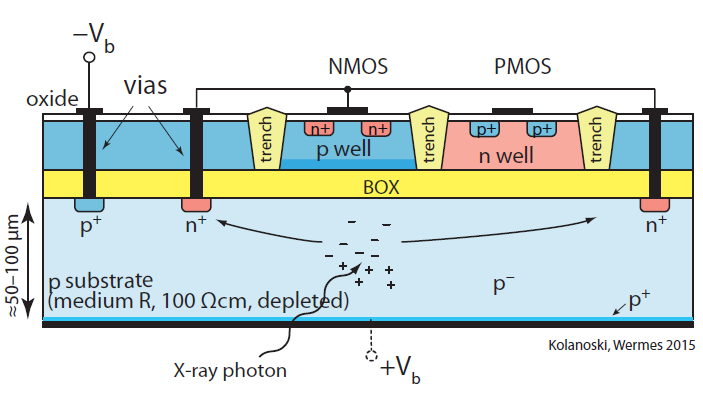
\includegraphics[scale=.7]{SOI_fig}
\caption{An example of a Monolithic SOI pixel.}
\label{fig:SOI_fig}
\end{figure}


\section{History of Monopix developments}

In recent years, advances in CMOS technologies have led to the development of a new generation of monolithic pixel sensors (DMAPS) with fast readout and high radiation tolerance. These new devices become promising candidate for high-energy physics experiment with high rates and high radiation environments.


\subsection{Developments of DMAP devices}

Specifically two different DMAPS development lines have been followed, distinguished by different pixel architectures, entrusted to two different implementation process technologies:


\begin{itemize}
\item \textbf{large fill factor} line: with large collection electrode and the electronics inside the charge collection well, these prototypes are indicate to experiments with high rate and high radiation conditions, because they could ensure a greater tolerance to huge doses of radiation. They have been fabricated in LFOUNDRY 150 nm design \cite{Barbero:2019bkw}. In~\autoref{fig:LF} are shown some of these chip developments.
\item \textbf{small fill factor} line: with small collection electrode and the electronics outside the charge collection well, these devices need a process modification to enhance the radiation hardness. They are faster compared to the previous type, and due to less values of total capacitance, they implicate much less power consumption. They are fabricated in a TowerJazz 180 nm CMOS imaging process.
\end{itemize}

\begin{figure}[h!]
\centering
\subfigure[CCPD\_LF]
{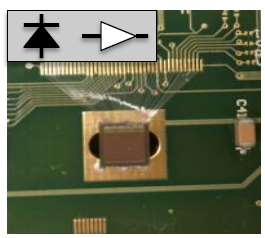
\includegraphics[scale=0.6]{LF1}}\quad
\subfigure[LF-CPIX]
{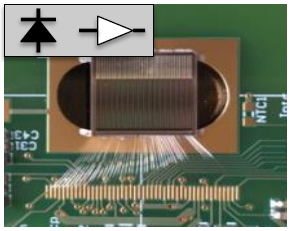
\includegraphics[scale=0.6]{LF2}}\quad
\subfigure[LF-MONOPIX 1]
{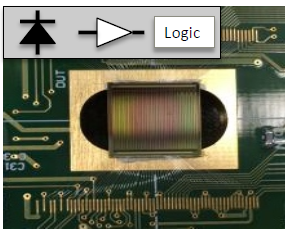
\includegraphics[scale=0.6]{LF3}}\\
\caption{LFOUNDRY 150 nm development line.}
\label{fig:LF}
\end{figure}


\subsection{TJ-Monopix line} \label{sec:TJ}

In~\autoref{fig:TJ} is displayed the TowerJazz development line that have allowed to design the last iteration of this series, TJ-Monopix2, whose characterization results will be shown in~\autoref{ch:TJ2}.\\

\begin{figure}[h!]
\centering
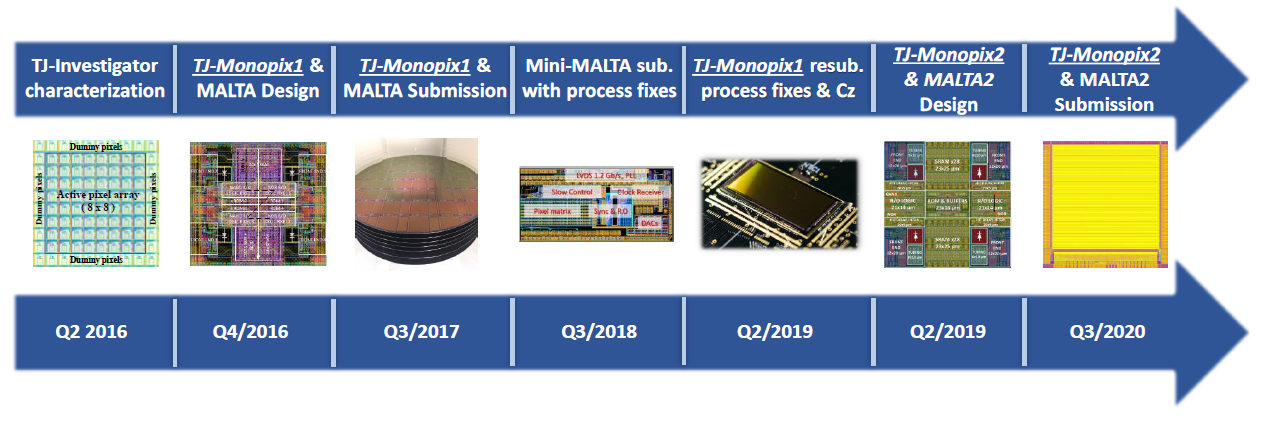
\includegraphics[scale=.55]{TJ}
\caption{TowerJazz 180 nm development line.}
\label{fig:TJ}
\end{figure}

The standard TowerJazz 180 nm process has been employed to realize the ALPIDE monolithic active pixel sensor, selected for the ALICE Inner Tracking System (ITS) upgrade \cite{ALICE:2013nwm}.

The chip proved to be suitable for the modest ALICE requirements, but the standard process do not ensure the full depletion volume, which is crucial to limit the signal degradation expecially after irradiation. For this reason, the aforementioned process modification have been developed by CERN in collaboration with the foundry \cite{SNOEYS201790}, that allows full depletion of sensitive layer. This new implementation has been tested in a dedicated chip called TJ-Investigator, and the obtained results have been demonstrated the effectiveness of the modified process. \\
Therefore two large scale demonstrator chips have been realized, called TJ-Monopix1 and TJ-Malta1 \cite{Moustakas:2017qqw}, whose main difference lies in the different readout architecture. The TJ-Malta1 chip implemented an \textit{asynchronous} readout architecture, which eliminate the Bunch Crossing ID (BCID, timestamp), in order to reduce the digital power consumption. For TJ-Monopix1 instead, a \textit{coulmn-drain} readout architecture was chosen, which will be described in the following. Both chips have been fully tested and irradiated to investigate their functionality and efficiency, which however has decreased from 97 \% to 70 \% after irradiation with an equivalent neutron fluence of \SI{e15}{n_{eq}/cm^{2}} \cite{Caicedo:2019lrk}. 

\begin{figure}[h!]
\centering
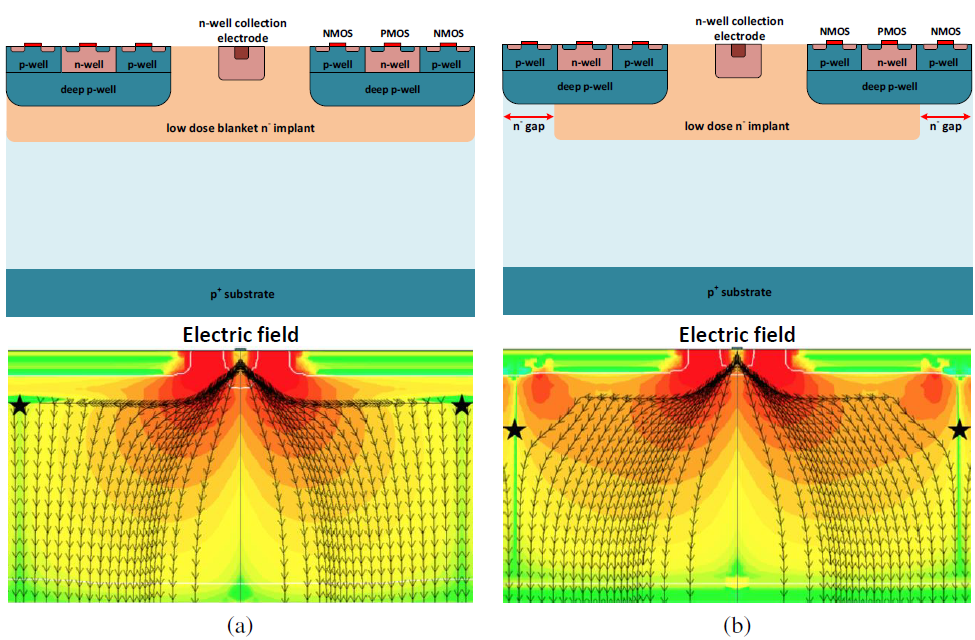
\includegraphics[scale=.7]{enhance_lateral}
\caption{In the left, the Full deep p-well (FDPW) structure and its lateral electric field, compared with te Removed deep p-well (RDPW) variation. Both of them implemented the process modification with a low dose n implant.}
\label{fig:enhance_lat}
\end{figure}


The main reason for the efficiency drop has been discovered to be related to the weak lateral electric field at the pixel edges. So the process has been further optimized in order to resolve this issue. Two different approaches were found to increase the lateral electric field at the pixel borders~\cite{Munker_2019}: creating a gap in the deep n-implant \textbf{n-gap} variant, requiring only a mask change, or introducing an additional p-type implant at the pixel border \textbf{extra deep p-well} variant. The n-gap variant is shown in~\autoref{fig:enhance_lat} compared to the previous version.

It can be seen the significant improvement of the electric lateral field, which results in turn in faster charge collection and so high efficiency even after irradiation. 

Further optimization of the pixel size, which is critical to take full advantage of field shaping through process modifications and to improve charge collection, have been implemented in the last iteration of this development line: TJ-Monopix2, considered as starting point for the development of the OBELIX final chip, designed for the upgrade of the Belle II vertex detector.  

Now we want to describe the analog circuit and the readout architecture chosen for TJ-Monopix2. 


\begin{description}
\item[The Column-drain readout architecture]
\end{description}

As we have seen in the previous, due to small capacitance of the small electrode MAPS, voltage amplification can be used to transform the charge signal arriving on the sensing node into a voltage signal. 

In~\autoref{fig:analog} a schematic of the voltage amplification and the readout stages.

\begin{figure}[h!]
\centering
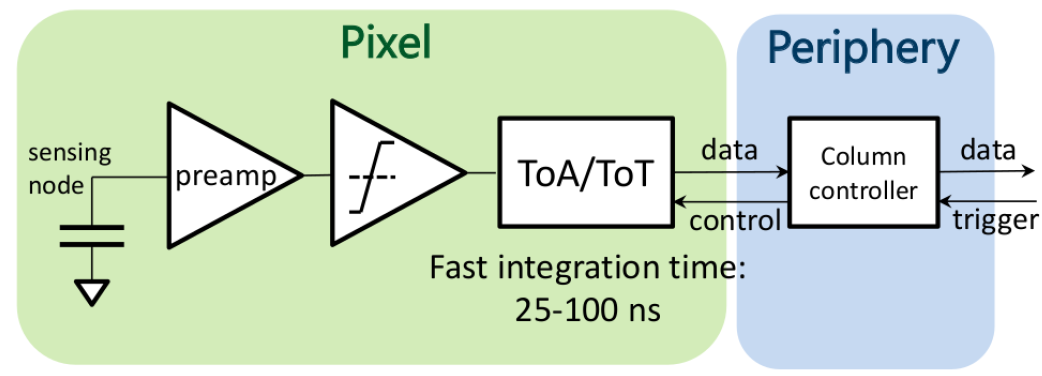
\includegraphics[scale=.5]{analog2}
\caption{Sketch of the voltage amplification stages and the readout.}
\label{fig:analog}
\end{figure}

The charge signal produced by particles passing through and collected by the collection node, is converted in a voltage signal through a small capacitance. It goes in input to a pre-amplifier which amplifies the signal and then send it to a discriminator. At this stage, the discriminator decides if discriminate the signal or not, on the base of its voltage threshold value. If the signal arriving from the pre-amplifier remains under the discriminator threshold, then it is not discriminate. If the signal goas above the threshold instead, the pulse is discriminate and its Time Over Threshold is measured (more about this in the following). Discriminator threshold is set by the means of some chip registers that we will see in \label{ch:TJ2}. Data collected are send to the periphery in order to comunicate and store them outside the chip.\\

\begin{figure}[h!]
\centering
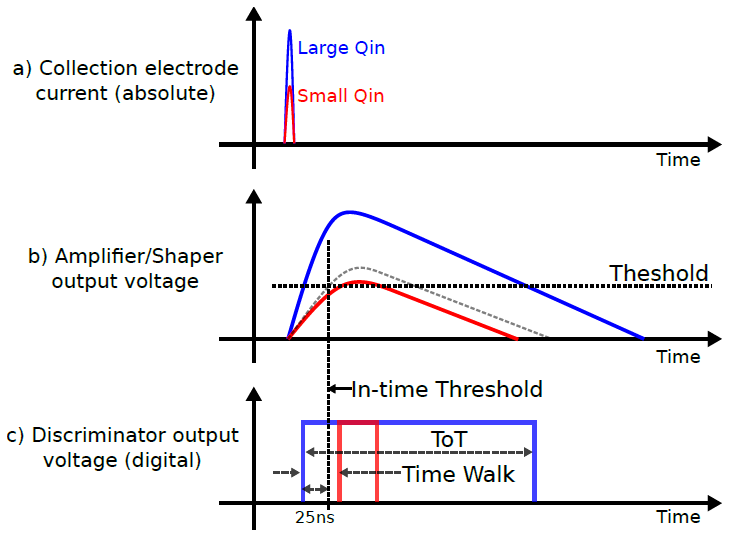
\includegraphics[scale=.7]{ToT}
\caption{Time Overt Threshold (ToT) technique.}
\label{fig:tot_scheme}
\end{figure}


The \textit{column-drain} architecture implemented in TJ-Monopix ensures fast readout by encoding the analog charge information using the standard \textbf{Time Over Threshold (ToT)} technique~\autoref{fig:tot_scheme}. This procedure exploits two timing information: the \textbf{Leading Edge (LE)} which corresponds to the hit time of arrival (when the signal value goes beyond the threshold), and the \textbf{Trailing Edge (TE)} that is when the signal goes below the threshold value. From the difference between the TE and the LE, the ToT can be calculated.  %(\autoref{fig:ToT}).

The \textit{in-pixel} circuitry implemented a Random Memory Acces (RAM) where to store the LE and TE timing info, a Read-Only Memory (ROM) to store the pixel address and the control and arbitration logic, which we will see more about in the following.
 
The readout is \textit{column-based}, so all pixels of each double column share a common column-bus which could be accessed by one pixel at a time, with a defined priority logic. The column bus includes the BCID timestamp, the data (LE, TE, address) and the control signals.
The \textit{periphery} includes the End Of Column (EoC) block which deals with the transmission and the readout of the column-bus signals, and the Digital Chip Bottom (DCB) that instead, processes the hit information. 

The readout could be triggered or full-readout. In TJ-Monopix line hit data is continuously transmitted to the DAQ. In case of triggered readout instead, hit data is stored in a trigger memory, and the information is transmitted only when the trigger signal arrives.

In~\autoref{fig:RO2} is displayed an example of the readout of two hits. 

\begin{figure}[h!]
\centering
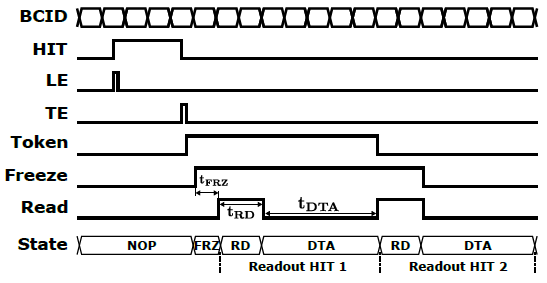
\includegraphics[scale=1]{RO2}
\caption{Schematic of a readout sequence where two hits are being processed.}
\label{fig:RO2}
\end{figure}

The readout sequence starts when the TE pulse arrived. A hit flag is set and it acivates the \textsc{\textbf{TOKEN}} signal, which in turn is arised to warn that the pixel is available to be read out. This signal propgates across the double column with a priority logic until it arrives to a readout controller, which uses other two global signals, the \textsc{\textbf{FREEZE}} and \textsc{\textbf{READ}}, to control the readout progression. They are distributed across the EoC blocks and local copies are transimitted only to the double column that has been hit and that has the higher priority (It is a different priority logic among each double column which goes from left to right across the matrix).
The first ensures that new hits do not interrupt the pixel priority logic setting other new hit flag, which means that they could not transmit new hit information, but they could store it for the next readout sequence. In this way the pixel priority in each readout sequence is well defined. The \textsc{\textbf{READ}} signal instead, allows to the pixel with the hit flag and highest priority to access the data bus and transmit the hit information to the periphery. A series of \textsc{\textbf{READ}} cycles allow all pixels in the sequence to be read out.


\begin{figure}[h!]
\centering
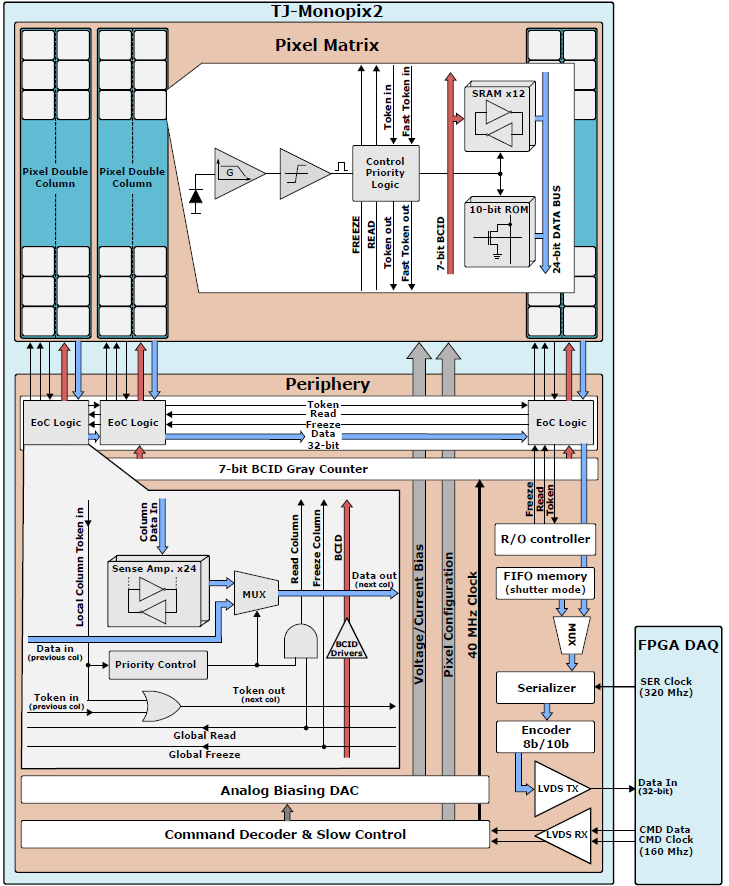
\includegraphics[scale=1]{RO}
\caption{Architecture of TJ-Monopix2.}
\label{fig:RO}
\end{figure}

%ROIC ReadOut Integrated Circuit
%occupancy
%energy necessary to release for silicon 3.65 e numero medio elettroni prodotti??
%other semiconductor


